\section{CIVIS Platform  Development} 
 
The development of the CIVIS platform started in May 2015 \citep{Huang2015c} and continued in the third year's WP3 activities. At the time of writing this deliverable (May/Jun 2016), the development is completed with minor updates took place in the past month.
% 
The JavaScript (JS) programming language\footnote{\url{http://www.crockford.com/javascript/javascript.html}} is used for development at both front- and back-ends. 
Figure~\ref{fig:ScreenShot2015-11-09at18} provides an overview of the major technologies used at the front-end and back-end. They are discussed in this section. 
The platforms and technologies mentioned are all free and open source. 

\begin{figure}
\centering
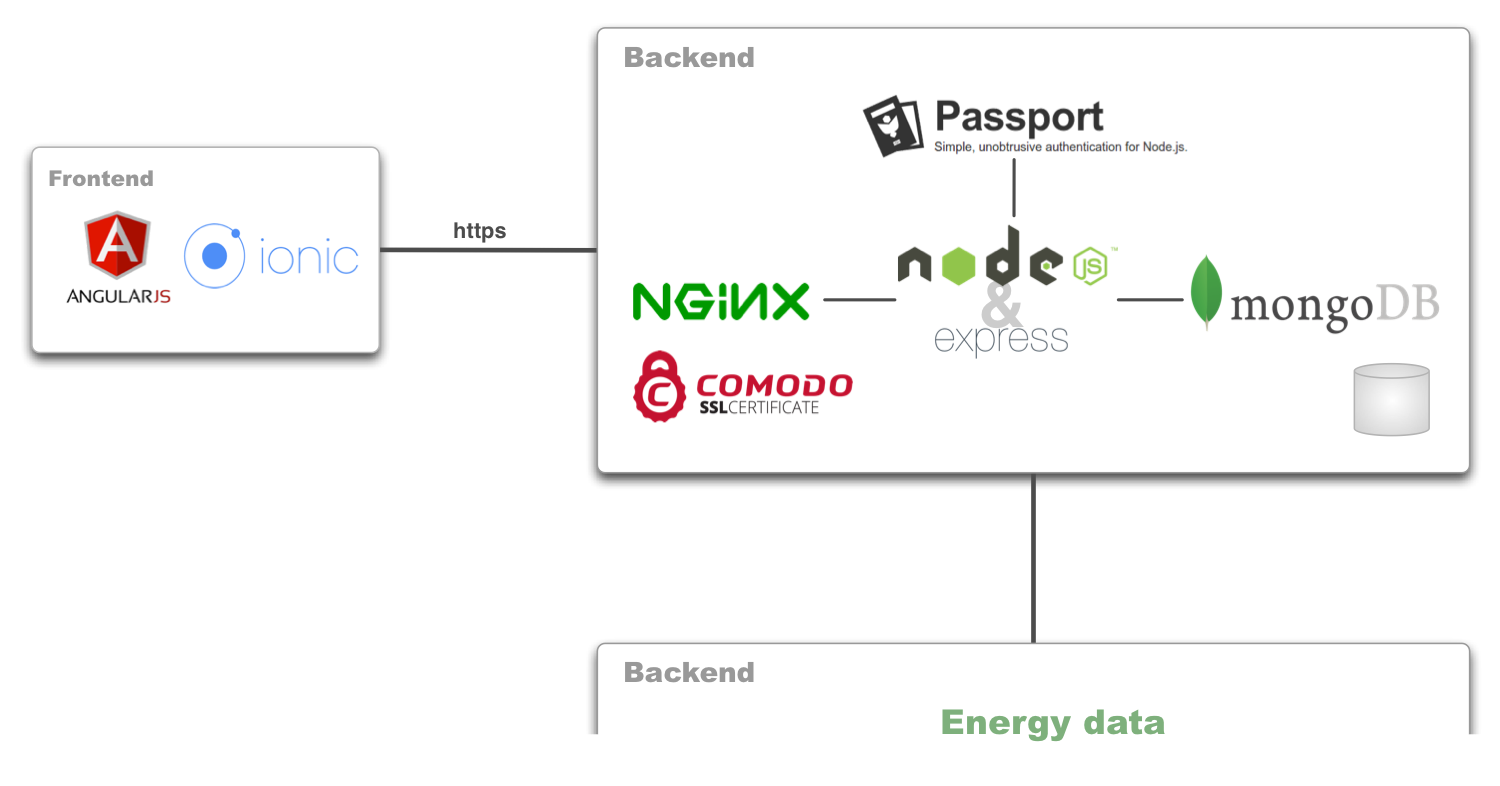
\includegraphics[width=0.9\linewidth]{img/tech}
\caption{WP3 front-end and back-end overview (``Energy data'' is covered by WP4)}
\label{fig:ScreenShot2015-11-09at18}
\end{figure}

\subsection{CIVIS Front-end as a Hybrid Application} 

The CIVIS front-end (YouPower) is developed as a hybrid (cross-platform) mobile application using \textit{Ionic}\footnote{\url{http://ionicframework.com/}}, an HTML5 front-end development framework built with SASS\footnote{\url{http://sass-lang.com/}} and optimized for AngularJS\footnote{\url{https://angularjs.org/}} (a.k.a Angular). 
% 
The Ionic framework comes with native-styled mobile UI elements and layouts, and handles the look and feel and the UI interactions the app needs in order to be compelling\footnote{\url{http://ionicframework.com/docs/guide/}}. 

Angular as a JS framework provides directives (extensions of HTML attributes) and two-way data binding (binds input or output data of the view to a model) that simplify the app development with Model-View-Controller (MVC) architecture. 
In two-way data binding, the value of a data model is passed on from the view (or loaded from the back-end) to the controller at run-time, and the function in the controller returns the result (of the value manipulation) to the view. 
% 
Other noteworthy JS and Angular libraries (i.e. besides Ionic) we use for the front-end development are as follows:

\begin{itemize}

\item Highcharts\footnote{\url{http://www.highcharts.com/}}, a charting library in JS. It provides an easy way to add interactive charts to the application. 

\item Highcharts-ng\footnote{\url{https://github.com/pablojim/highcharts-ng}}, a simple Angular directive for Highcharts. 

\item Angular-translate\footnote{\url{https://angular-translate.github.io/}}, an Angular module for internationalization and localization of the application. (YouPower is currently available in English, Swedish and Italian.)

\item Angular-resource\footnote{\url{https://docs.angularjs.org/api/ngResource}}, an Angular module for interacting with RESTful server-side data sources. 

\item Underscore.js\footnote{\url{http://underscorejs.org/}}, a JS library that provides over 100 utility functions. 

\item Bootstrap-sass\footnote{\url{https://github.com/twbs/bootstrap-sass}}, a Sass-powered version of Bootstrap 3. 

\item Moment.js\footnote{\url{http://momentjs.com/}}, a JS library to parse, validate, manipulate and display dates. 

\item Ion-datetime-picker\footnote{\url{https://www.npmjs.com/package/ionic-datetime-picker}}, a date and time picker for the ionic framework. 

\end{itemize}


\subsection{CIVIS Back-end as a JS Runtime Environment}

The YouPower back-end is developed using the \textit{Node.js}\footnote{\url{https://nodejs.org/}} platform, a well-known JS based open source runtime environment for server-side applications. 
The platform is easily extensible and has a repository of libraries that support fast web development. 
% 
TU Delft prepared a virtual machine for CIVIS to host the WP3 back-end\footnote{\url{http://civis.tbm.tudelft.nl}}
using \textit{Nginx}\footnote{\url{https://nginx.org/en/}}, an http and reservse proxy server. 
% 
A \textit{Comodo}\footnote{\url{https://ssl.comodo.com/}} SSL certificate is installed on the server to provide secure communication (i.e. https). 

% 
The WP3 back-end interacts with the WP4 back-end, from which the former fetches relevant energy data that is particularly relevant for visualization of energy consumption/production and energy consumption signal. The availability of such data through the WP4 platform represents therefore a pre-condition for the ability of the app to correctly visualize such information.

\textit{MongoDB}\footnote{\url{https://mongodb.org/}} is used as the back-end database. It is document-oriented, and has flexible data schema and expressive query language. 
A list of the data models at the back-end can be found at {\footnotesize\url{https://github.com/CIVIS-project/YouPower/tree/master/backend/models}}. 
Figure~\ref{fig:datamodel} shows the data model schema.
%
\begin{figure}
\centering
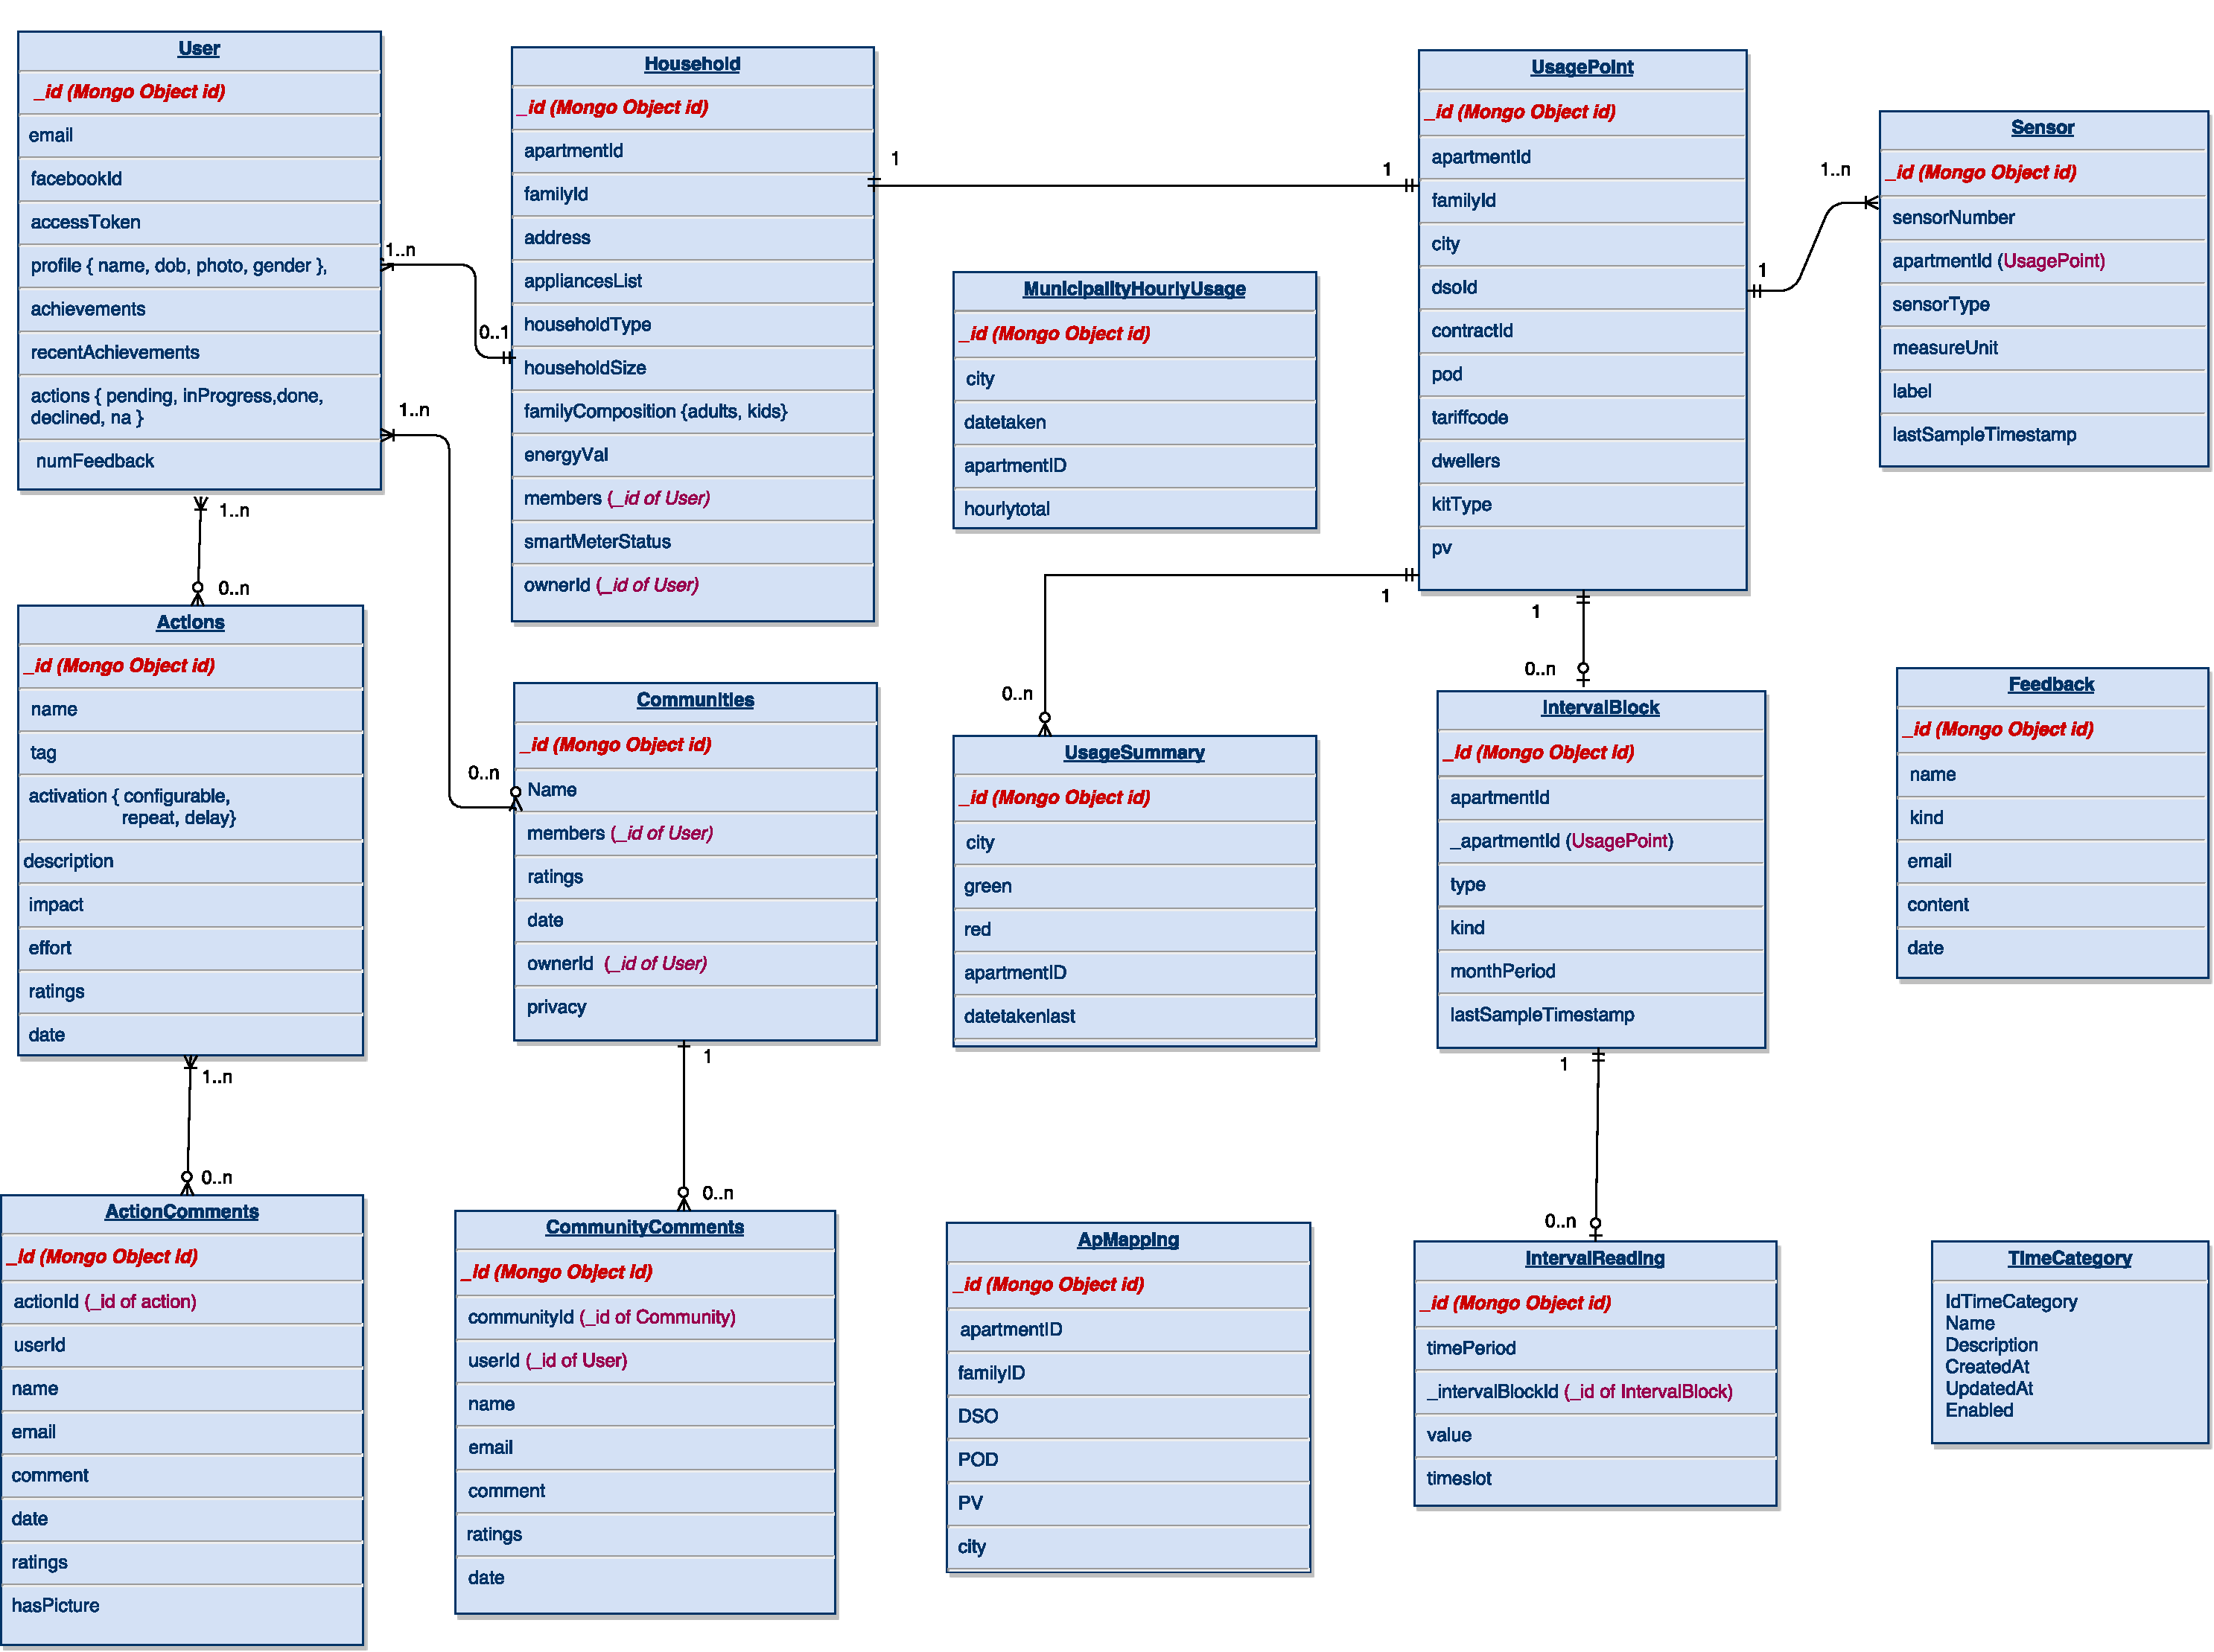
\includegraphics[height=.92\linewidth,angle=90]{img/7sdatamodel}
\caption{YouPower back-end data model schema}
\label{fig:datamodel}
\end{figure} 
% 

The noteworthy Node.js libraries used for the WP3 back-end development are as follows:

\begin{itemize}

\item Async.js\footnote{\url{https://github.com/caolan/async}}, which makes managing and combining asynchronous tasks easier. 

\item Express.js\footnote{\url{http://expressjs.com/}}, a Node.js application server framework we use as a basis for the REST API. 

\item Mocha\footnote{\url{https://mochajs.org/}}, a JavaScript unit test framework. 

\item Mongoose\footnote{\url{http://mongoosejs.com/}}, a MongoDB driver for Node.js. It provides a schema-based solution to model data. 

\item Passport.js\footnote{\url{http://passportjs.org/}}, for handling authentication of REST API requests for Node.js, both local (username password) and Facebook. 

\item Underscore.js\footnote{\url{http://underscorejs.org/}}, a JS library that provides over 100 utility functions. 
%\item Ionic Push\footnote{\url{https://apps.ionic.io/landing/push}}, for sending dynamic push notifications. 

\item Nodemailer\footnote{\url{https://nodemailer.com/}}, sending emails with Node.js.

\item Email-templates\footnote{\url{https://www.npmjs.com/package/email-templates}}, a Node.js module for rendering beautiful emails.

\item Fb\footnote{\url{https://www.npmjs.com/package/fb}}, a Node.js library for Facebook.

\item Moment.js\footnote{\url{http://momentjs.com/}}, a JS library to parse, validate, manipulate and display dates. 

\item APIDOC script\footnote{\url{http://apidocjs.com/}}, for inline documentation for the REST API. 
\item node-xml2js\footnote{\url{https://github.com/Leonidas-from-XIV/node-xml2js}}, Simple XML to JavaScript object converter. 
\item dateformat\footnote{\url{https://www.npmjs.com/package/dateformat}}, for formatting dates to custom formats. 
\item HTTPS\footnote{\url{https://nodejs.org/api/https.html}}, A nodeJs module used to make service calls over TLS/SSL. 
\item querystring\footnote{\url{https://www.npmjs.com/package/querystring}}, for deserializing querystring to an object. 
\item fs\footnote{\url{https://www.npmjs.com/package/querystring}}, for manipulating file in NodeJS. 
\end{itemize}

The YouPower back-end REST API documentation can be found at {\footnotesize\url{http://civis.tbm.tudelft.nl/apidoc/}}. 
% 

\subsection{Resources}

\subsection{Package Management}

\begin{itemize}

\item Bower\footnote{\url{http://bower.io/}}, a package manager for the front-end development to keep track of and update the packages. 

\item Gulp\footnote{\url{http://gulpjs.com/}}, a toolkit that helps to automate tasks in the development work-flow. 

\item 

\end{itemize}